% \section{Results}
\section{Resultados}

% --- EFFECTIVE SAMPLE SIZE ---
\begin{frame}[c]{Tamaños Efectivos de Muestra}
  \begin{columns}[b]
    % --- LEFT COLUMN ----
    \begin{column}{0.64\textwidth}
      \centering
      
\includegraphics[width=\linewidth]{img/results/2026-02/effective-sample-sizes_robust-estimator_sibpair-trios.png}
    \end{column}
    % --- RIGHT COLUMN ----
    \begin{column}{0.36\textwidth}
      % --- UPPER QUADRANT ----
      \small\sffamily

      El estimador robusto tiene un mayor poder estadístico
      que el modelo de \textcite{young2022-fgwas}

      % --- LOWER QUADRANT ----
      \vspace{1cm}
      \vfill
      \captionof{figure}{
        \textbf{Comparación de tamaños efectivos de muestra para todos los rasgos en dos estimadores de FGWAS.}
        El estimador robusto vs. de pares de hermanos y trios parentales,
        incremento de 36.58\% (SD $\pm$ 6.78\%).
        Barras de error representan intervalos de confianza del 95\%.
      }
    \end{column}
  \end{columns}
\end{frame}

% --- HERITABILITY ---
\begin{frame}[c]{Comparación entre estimaciones de heredabilidad}
\begin{figure}
    \begin{minipage}[b]{0.67\textwidth}
        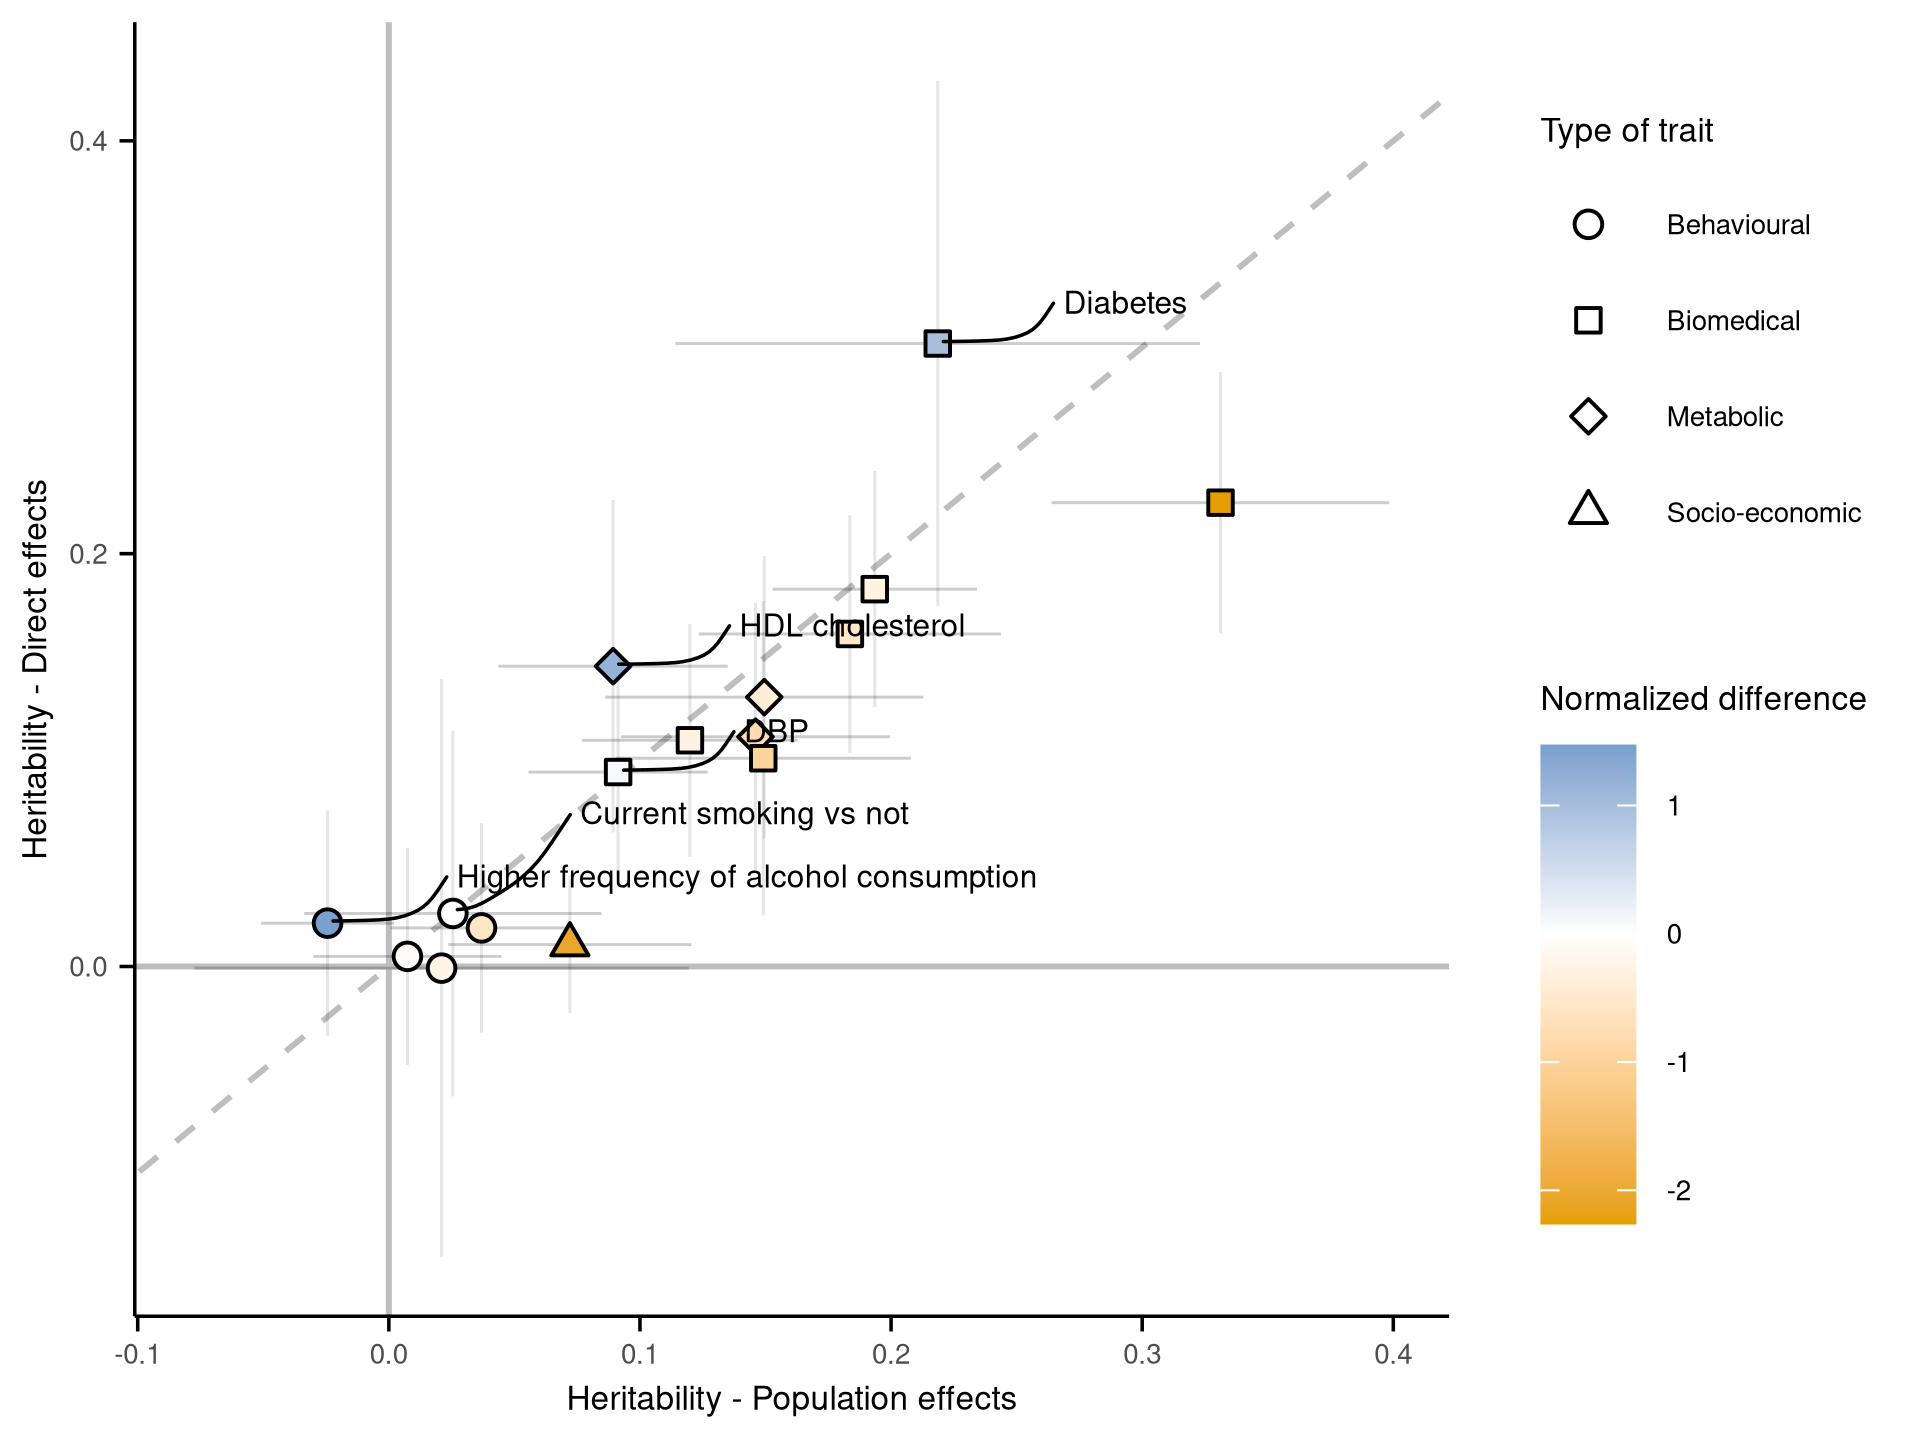
\includegraphics[width=0.95\textwidth]{img/results/2027-01/heritability/heritability_comparison.scatter.png}
    \end{minipage}\hfill
    \begin{minipage}[b]{0.33\textwidth}
        \caption{
            \textbf{Comparación de estimaciones de heredabilidad derivadas de FGWAS contra PopGWAS.}
            Cada punto representa un rasgo complejo.
            Los colores representan la clasificación.
            La línea punteada representa la línea de identidad.
            Barras de error representan intervalos de confianza al 95\%.
        }
    \end{minipage}
\end{figure}
\end{frame}

\begin{frame}[b]{Comparación de prevalencias entre subcohortes}
  \begin{figure}[htpb]
      \centering
      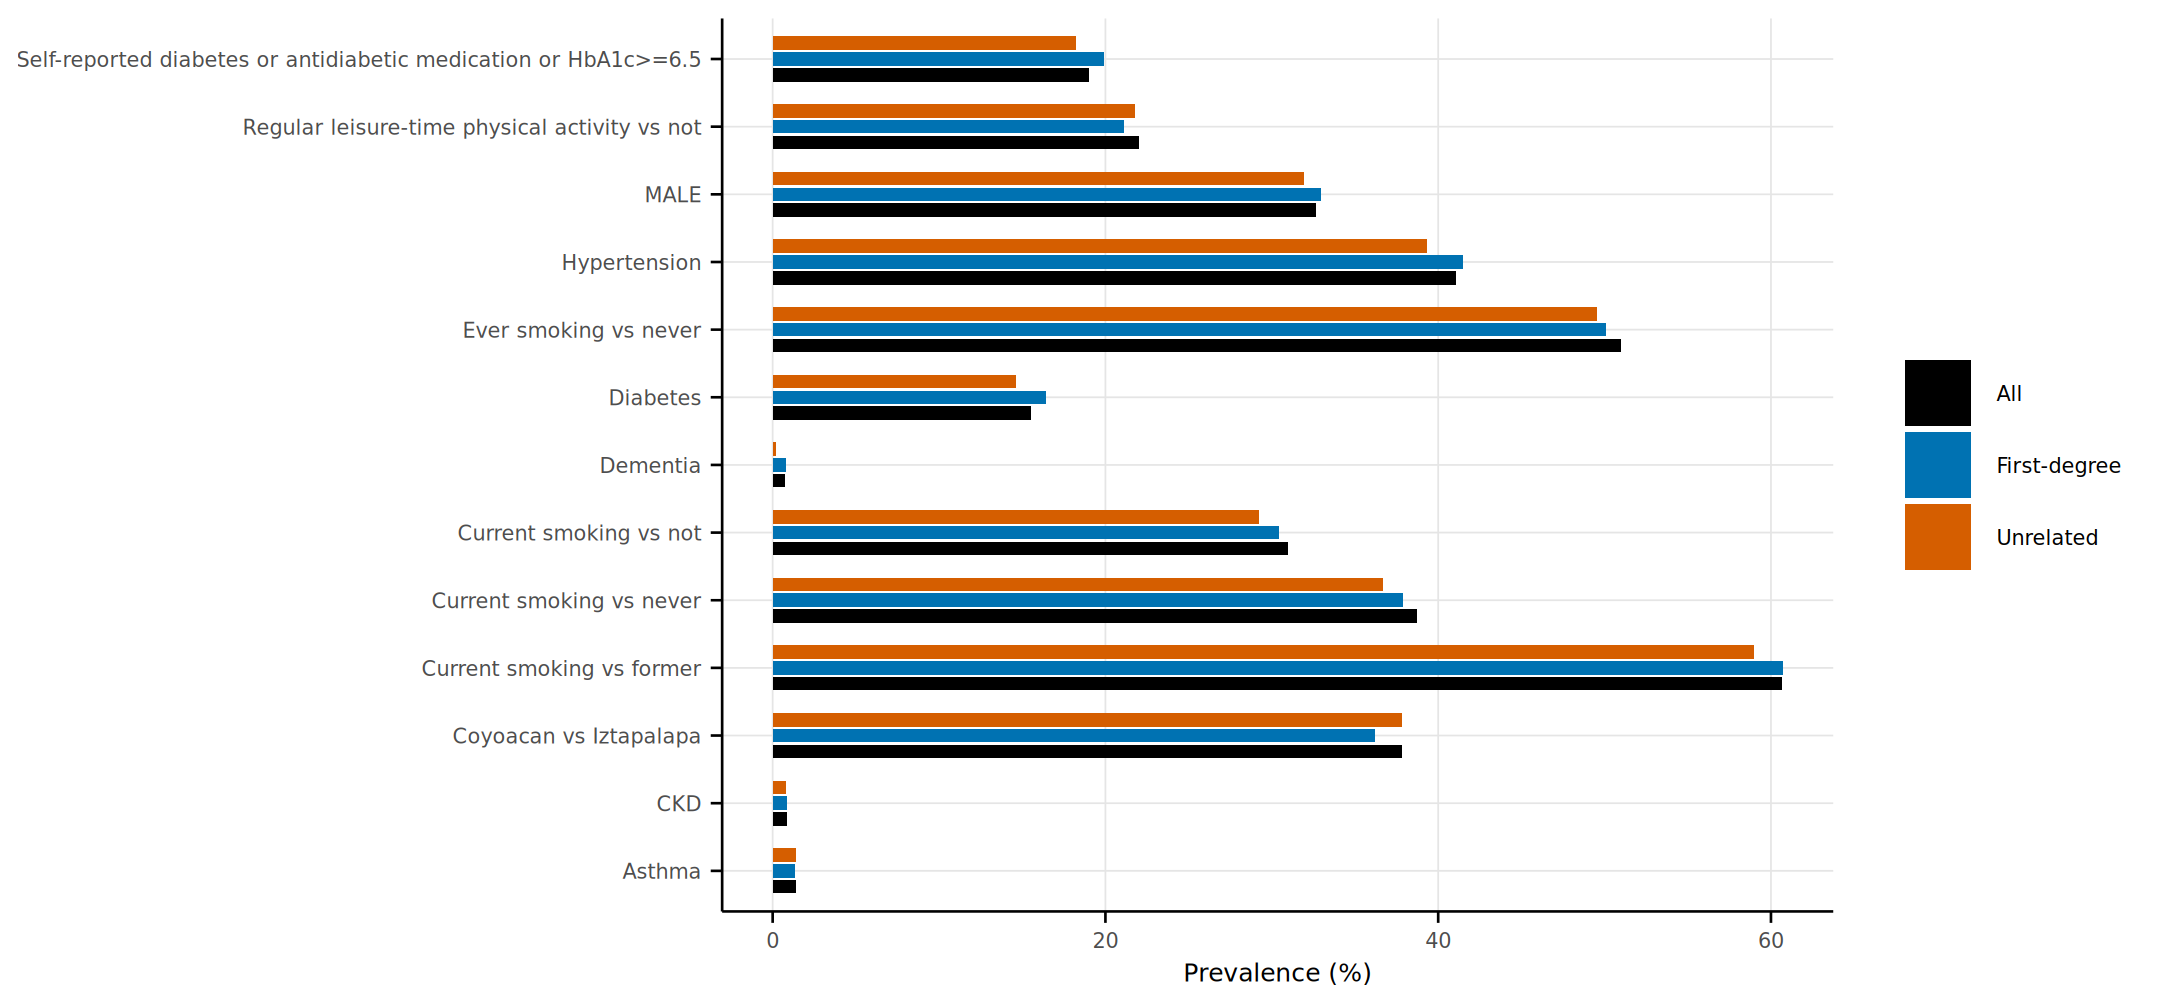
\includegraphics[width=0.9\textwidth, height=0.75\textheight, keepaspectratio]{img/results/2027-01/phenotype-smd-analyses/prevalence_comparison.cropped.png}
      \caption{
        \textbf{Comparación de prevalencias.} Prevalencias de fenotipos por subcohorte. \parencite{young2022-fgwas}
      }
      \label{fig:prevalences}
  \end{figure}
\end{frame}

\begin{frame}[c]{Comparación entre estimaciones de heredabilidad}
  \begin{figure}[htpb]
      \centering
      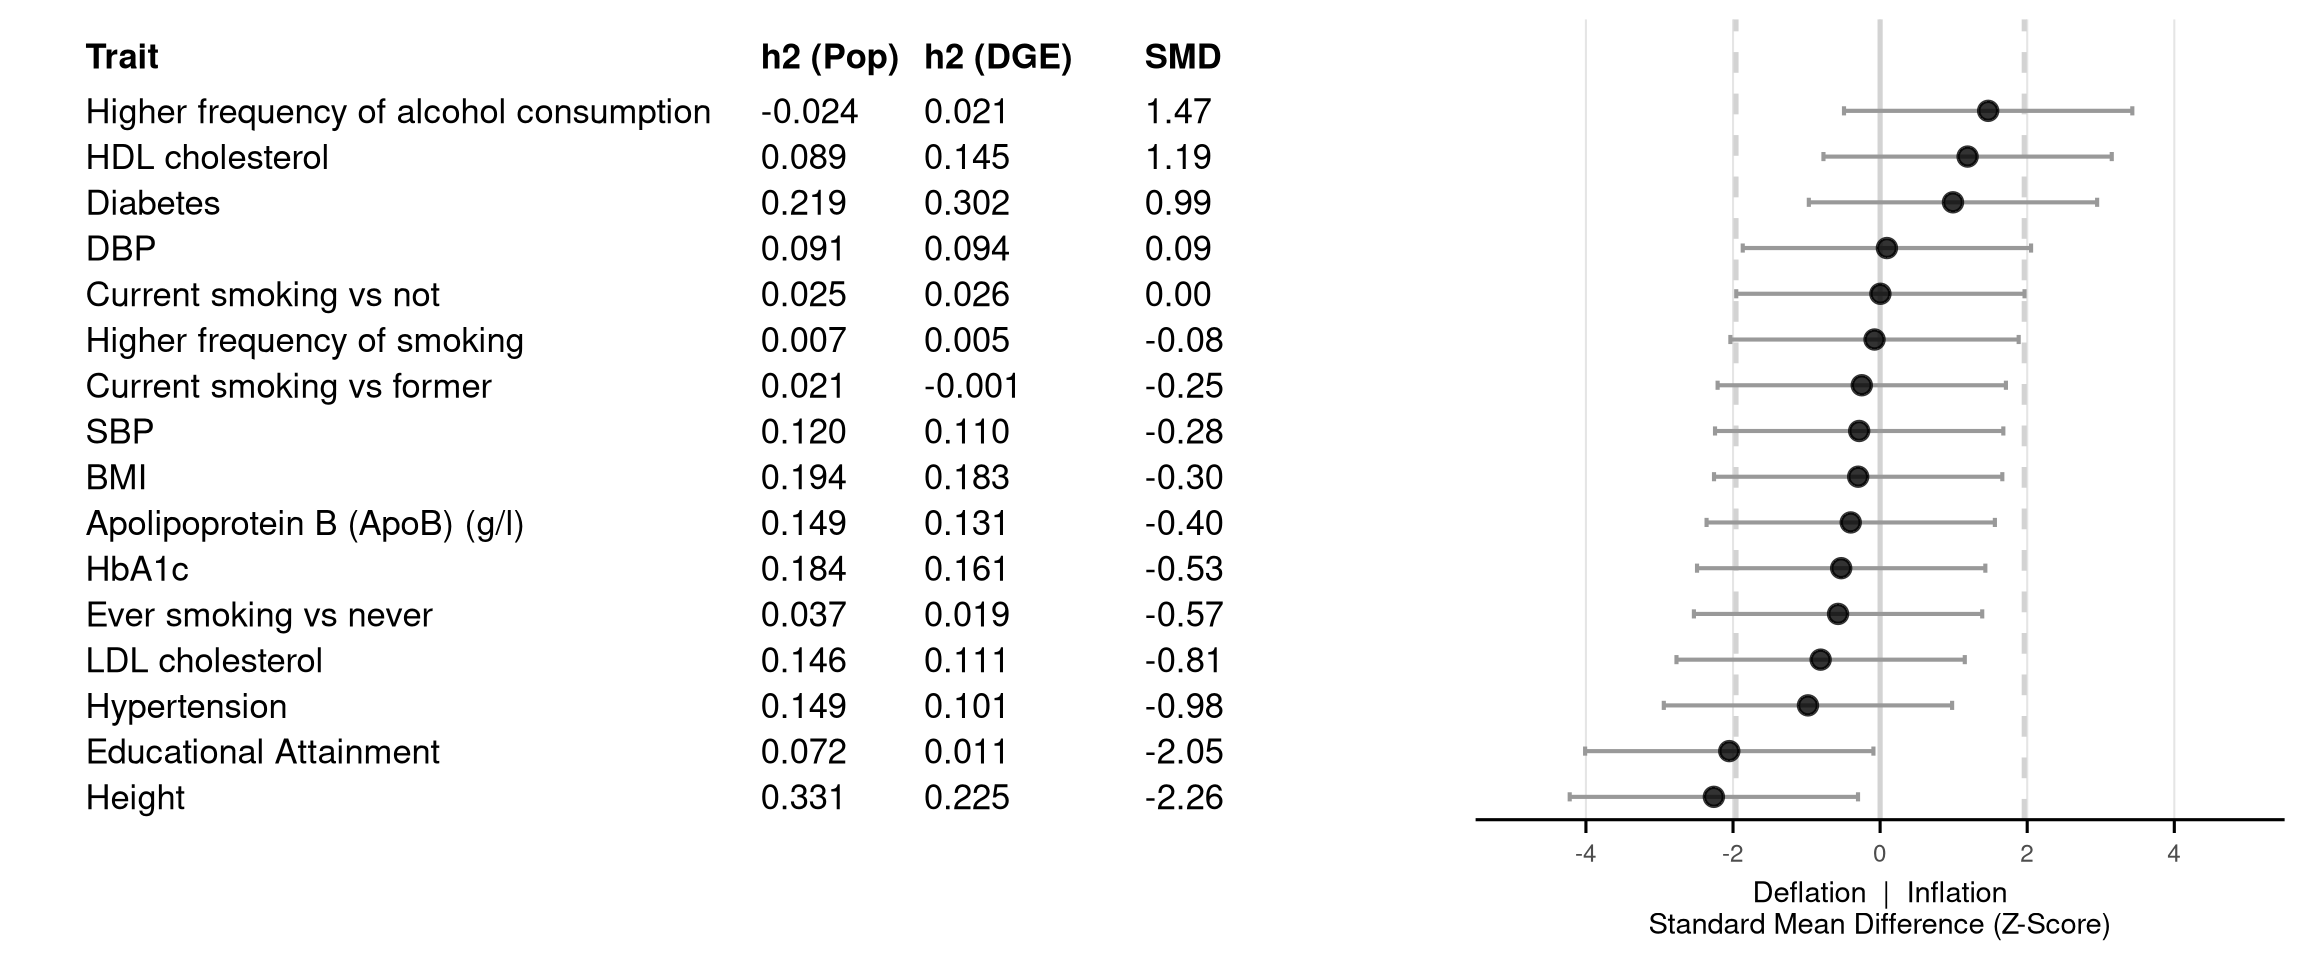
\includegraphics[width=0.9\textwidth, height=0.75\textheight, keepaspectratio]{img/results/2027-01/heritability/heritability_comparison.smd.png}
      \caption{
        \textbf{Diferencias normalizadas entre estimaciones de heredabilidad.} Las lineas verticales en la gráfica indican CI 95\%.
      }
      \label{fig:h2-smd}
  \end{figure}
\end{frame}

\begin{frame}[b]{Las subcohortes tiene diferencias sistemáticas por sesgos de averiguación}
  \begin{figure}[htpb]
      \centering
      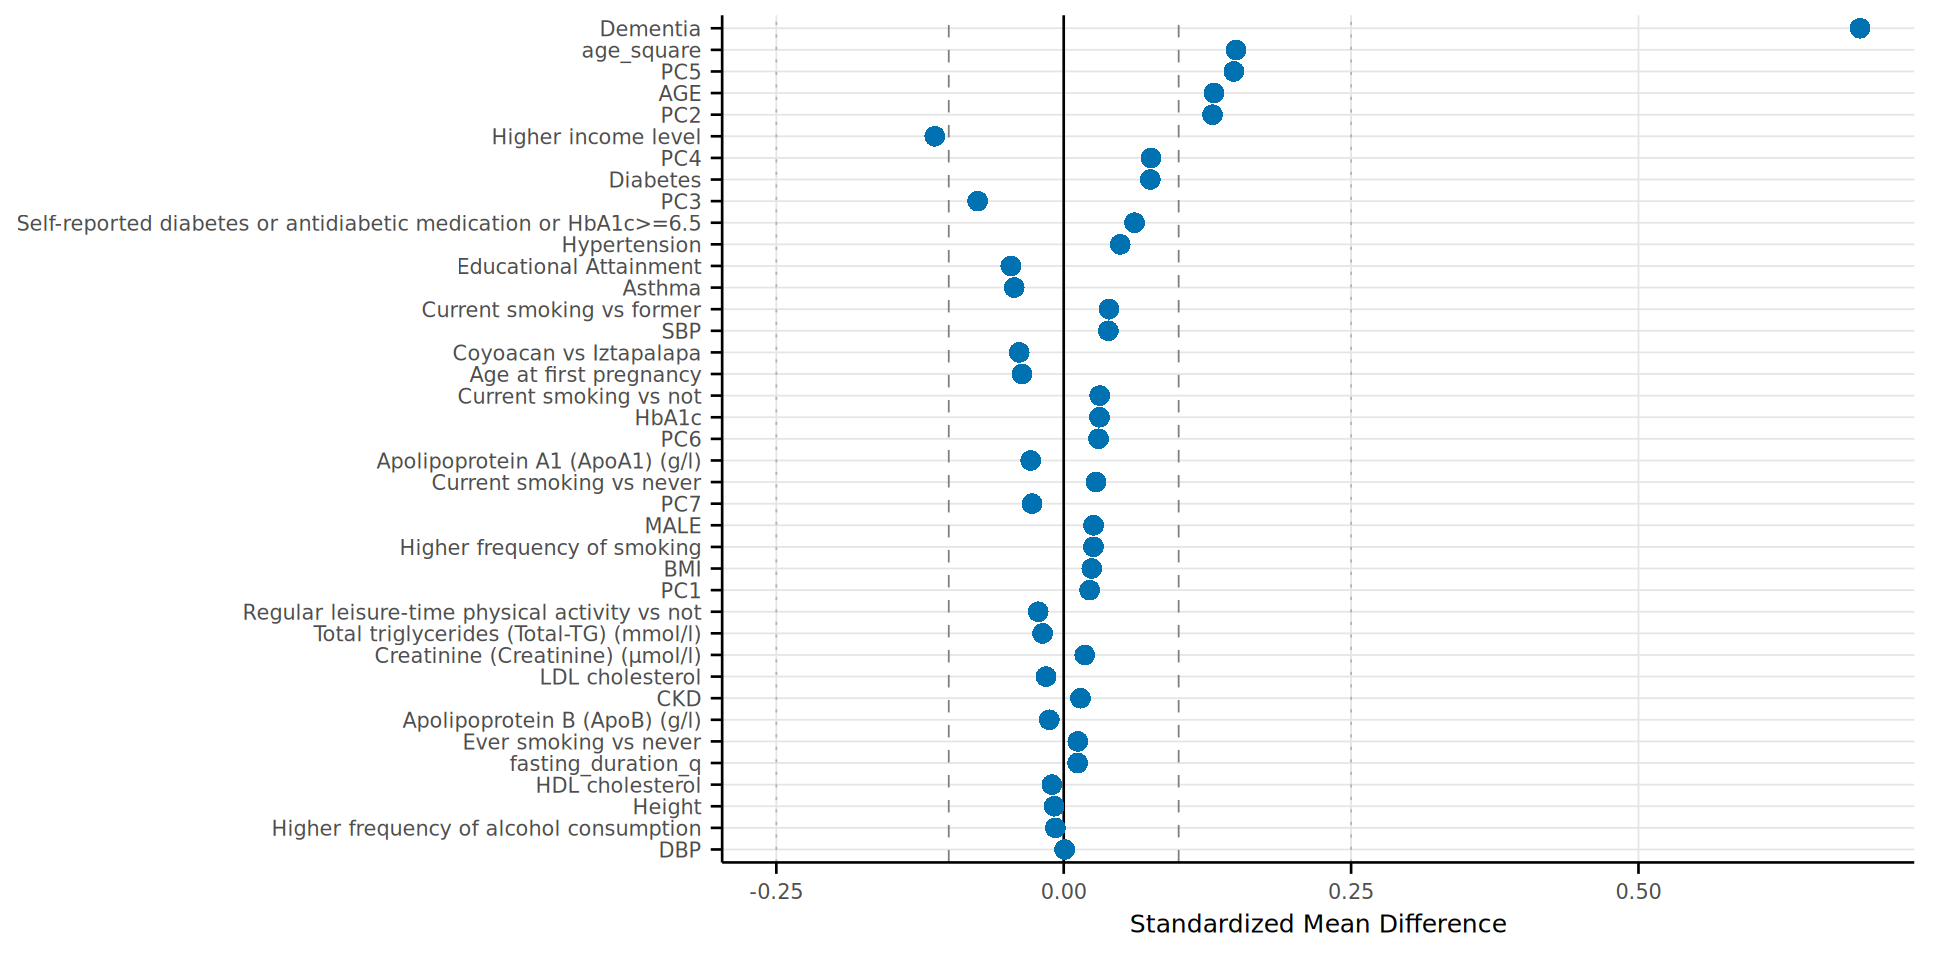
\includegraphics[width=0.9\textwidth, height=0.75\textheight, keepaspectratio]{img/results/2027-01/phenotype-smd-analyses/forest_smd_bias_assessment_cropped.png}
      \caption{
        \textbf{Diferencias por sesgos de averiguación.} Diferencias de medias estandarizadas (SMD) entre subcohortes.
      }
      \label{fig:bias_assessment}
  \end{figure}
\end{frame}

\begin{frame}[c]{Atenuación a nivel de \textit{locus} independientes (Clumping)}
  \begin{table}[htpb]
      \centering
      \resizebox{\textwidth}{!}{
      \begin{tabular}{llllrrlp{4.5cm}}
          \toprule
          \textbf{Fenotipo} & \textbf{SNP} & \textbf{Gen} & \textbf{PopGWAS} $\beta$ & \textbf{FGWAS} $\beta$ & $\Delta \beta$ & \textbf{FDR} & \textbf{Patrón de Atenuación} \\
          \midrule
          Diabetes & \texttt{chr6:20660459:G:A} & \textit{CDKAL1} & -0.178 & -0.010 & -0.168 & $1.4 \times 10^{-8}$ & \textbf{Alto:} Gran efecto poblacional; efecto directo cercano a cero. \\
          Diabetes & \texttt{chr9:22137686:T:G} & \textit{CDKN2B} & -0.163 & -0.009 & -0.154 & $5.2 \times 10^{-8}$ & \textbf{Alto:} Asociación inflada por sesgos/confusión. \\
          LDL & \texttt{chr5:156924336:T:C} & \textit{TIMD4} & -0.049 & -0.016 & -0.032 & 0.145 & \textbf{Fuerte:} Efecto directo $\sim 3\times$ menor. \\
          Estatura & \texttt{chr7:44189469:C:T} & \textit{GCK} & -0.094 & -0.077 & -0.017 & 0.899 & \textbf{Moderado:} Efecto conservado, ligera sobreestimación. \\
          HbA1c & \texttt{chr19:44908822:C:T} & \textit{APOE} & 0.498 & 0.481 & 0.017 & 0.966 & \textbf{Estable:} Efecto directo robusto, mínima confusión. \\
          \bottomrule
      \end{tabular}
      }
      \caption{
        \textbf{Resumen de atenuación en \textit{loci} representativos (PopGWAS vs FGWAS).}
      }
      \label{tab:clumping_attenuation}
  \end{table}
\end{frame}

\begin{frame}[c]{Frecuencias alélicas por ancestría continental (MCPS)}
  \begin{table}[htpb]
      \centering
      \begin{tabular}{llrrr}
          \toprule
          \textbf{Gen} & \textbf{\textit{locus}} & \textbf{Freq. IMX} & \textbf{Freq. EUR} & \textbf{$\Delta$ (IMX - EUR)} \\
          \midrule
          \textit{CDKAL1} & \texttt{chr6:20660459:G:A} & 25.6\% & 34.2\% & $-8.6\%$ \\
          \textit{CDKN2B} & \texttt{chr9:22137686:T:G} & 34.1\% & 29.8\% & $+4.3\%$ \\
          \textit{GCK} & \texttt{chr7:44189469:C:T} & 19.3\% & 20.5\% & $-1.2\%$ \\
          \textit{TIMD4} & \texttt{chr5:156924336:T:C} & 53.0\% & 30.0\% & $+23.0\%$ \\
          \bottomrule
      \end{tabular}
      \caption{
        \textbf{Frecuencias alélicas en subpoblaciones de MCPS.} IMX = Indígena Americano, EUR = Europeo. Datos extraídos del MCPS Allele Frequency Browser (\url{https://rgc-mcps.regeneron.com/home}).
      }
  \end{table}
\end{frame}

\begin{frame}[t]{Conclusiones: Relevancia de los Modelos Familiares}
  \begin{columns}[T]
      \begin{column}{0.31\textwidth}
          \begin{block}{1. Diagnóstico de Sesgos}
              Los GWAS familiares operan como herramientas diagnósticas que permiten determinar la dirección y magnitud de sesgos en diseños de descubrimiento (PopGWAS), más que como estrategias primarias para identificación de \textit{loci}.
          \end{block}
      \end{column}
      \begin{column}{0.31\textwidth}
          \begin{block}{2. Poder Estadístico en MCPS}
              La implementación del estimador robusto incrementa eficientemente el tamaño de muestra efectivo frente a alternativas intra-familiares, permitiendo documentar rigurosamente efectos de composición ambiental en la cohorte.
          \end{block}
      \end{column}
      \begin{column}{0.33\textwidth}
          \begin{block}{3. Predicción de Riesgo (PRS)}
              Históricamente, construir puntajes poligénicos con estimaciones de FGWAS no ha mejorado la precisión predictiva. Sin embargo, evaluar empíricamente esta aproximación en población mexicana es un paso necesario para consolidar la evidencia.
          \end{block}
      \end{column}
  \end{columns}
\end{frame}

\begin{frame}[c]{Ancestría y Confusión Ambiental en Diabetes}
  \begin{itemize}
      \item<1-> Diabetes mellitus: fenotipo crítico con los mayores niveles de sesgo poblacional empírico.
      \item<2-> \textcite{torres2026-diabetes, wang2025-mcps}: La ancestría mexicana explica la alta prevalencia de la enfermedad.
      \item<3-> Estimadores intrafamiliares identifican \textbf{falsos positivos} en \textit{loci} canónicos de diabetes por confusión ambiental. % ponytail: directo al grano
      \item<4-> Urge el desarrollo de herramientas genómicas de mayor precisión para México.
  \end{itemize}
\end{frame}
